\documentclass[aspectratio=169,10pt]{beamer}
\usepackage[utf8]{inputenc}
\usepackage[T1]{fontenc}
\usepackage[english]{babel}
\usepackage{tikz}
\usepackage{listings}
\usepackage{amsmath,amssymb}
\usetikzlibrary{arrows.meta,positioning,shapes.geometric,calc,fit,backgrounds}

\usetheme{metropolis}
%\usetheme{focus}
%\setbeamertemplate{navigation symbols}{}

% ---------- colors ----------
\definecolor{rtblue}{RGB}{31,97,163}
\definecolor{rtgreen}{RGB}{46,139,87}
\definecolor{rtred}{RGB}{200,50,50}
\definecolor{rtorange}{RGB}{230,140,30}
\definecolor{rtgray}{RGB}{110,110,110}

\lstset{
  basicstyle=\ttfamily\scriptsize,
  keywordstyle=\color{rtblue}\bfseries,
  commentstyle=\color{rtgray}\itshape,
  language=C++,
  breaklines=true,
  frame=single,
  rulecolor=\color{rtgray},
  showstringspaces=false,
  moredelim=**[is][\color{rtred}\bfseries]{@}{@} % @...@ = highlighted
}

\tikzset{
  box/.style={draw,rounded corners=2pt,fill=#1!15,minimum height=0.8cm,align=center,font=\small},
  box/.default=rtblue,
  arr/.style={-{Stealth[length=2.5mm]},thick}
}
\usepackage{lmodern}
\setbeamertemplate{itemize item}{$\square$}
\setbeamertemplate{itemize subitem}{$\square$}
\setbeamertemplate{itemize subsubitem}{$\square$}

\setlength{\labelsep}{0.6em}

% Placeholder for figures you still have to produce
\newcommand{\figplaceholder}[3]{% file, size, caption
  \IfFileExists{#1}{\includegraphics[width=#2]{#1}}{%
    \begin{tikzpicture}\node[draw,dashed,rtgray,minimum width=#2,minimum height=3cm,align=center,font=\small]
    {\textbf{TODO figure}\\#3};\end{tikzpicture}}}
\newcommand{\bol}[1]{\boldsymbol{#1}}
\newcommand{\dd}{\,\mathrm{d}}
\title{Visibility via GPU Ray Tracing}
\subtitle{Visibility matrix of a 3D mesh with OptiX and RT Cores, coupled to FreeFEM++}
\author{FreeFEM++ / CUDA / OptiX project}
\date{}

\begin{document}

\begin{frame}\titlepage\end{frame}

\begin{frame}{Outline}\tableofcontents\end{frame}

%=====================================================================
\section{Motivation and application}
%=====================================================================
\begin{frame}{Application: surface exchange between red blood cells}
  \begin{columns}[T]
    \begin{column}{0.5\textwidth}
      \figplaceholder{mesh_rbc.png}{\textwidth}{3D mesh, triangles coloured by label (RBC vs.\ domain boundary)}
    \end{column}
    \begin{column}{0.48\textwidth}
      \begin{itemize}
        \item 3D FreeFEM++ mesh; boundary triangles $T_1,\dots,T_N$.
        \item Triangles with a label in \texttt{rbcLabels} are \alert{obstacles}.
        \item Two triangles \alert{exchange} only if they see each other.
        \item Coupling term (view factor type):
        \[ \sum_{j} V_{ij}\, F_{ij}\,(u_j-u_i) \]
        \item $V_{ij}\in\{0,1\}$: visibility. \textbf{TODO:} state your actual equation here.
      \end{itemize}
    \end{column}
  \end{columns}
  \vspace{1mm}
  \begin{alertblock}{Goal}
    Compute $V\in\{0,1\}^{N\times N}$ fast enough to be used inside a simulation.
  \end{alertblock}
\end{frame}

\begin{frame}{The problem: who sees whom?}
  \begin{columns}[T]
    \begin{column}{0.52\textwidth}
      \[ V_{ij}=1 \iff \text{segment } [g_i,g_j] \text{ crosses no obstacle} \]
      \begin{itemize}
        \item $g_i$: barycenter of triangle $i$.
        \item One pair = one \alert{ray} to test against the obstacles.
        \item $V$ symmetric, zero diagonal: only $i<j$.
      \end{itemize}
    \end{column}
    \begin{column}{0.46\textwidth}
      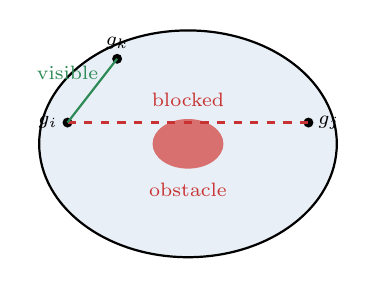
\begin{tikzpicture}[scale=0.9]
        \draw[thick,fill=rtblue!10] (0,0) ellipse (2.1 and 1.6);
        \fill[rtred!70] (0,0) ellipse (0.5 and 0.35);
        \node[font=\scriptsize,rtred] at (0,-0.65) {obstacle};
        \fill (-1.7,0.3) circle (2pt) node[left,font=\scriptsize] {$g_i$};
        \fill (1.7,0.3) circle (2pt) node[right,font=\scriptsize] {$g_j$};
        \fill (-1.0,1.2) circle (2pt) node[above,font=\scriptsize] {$g_k$};
        \draw[rtred,dashed,thick] (-1.7,0.3) -- (1.7,0.3);
        \node[rtred,font=\scriptsize] at (0,0.62) {blocked};
        \draw[rtgreen,thick] (-1.7,0.3) -- (-1.0,1.2);
        \node[rtgreen,font=\scriptsize] at (-1.7,1.0) {visible};
      \end{tikzpicture}
    \end{column}
  \end{columns}
\end{frame}

%=====================================================================
\section{The computational challenge}
%=====================================================================
\begin{frame}{The quadratic wall}
  \[ \text{numPairs}=\frac{N(N-1)}{2}, \qquad \text{brute force}=\frac{N(N-1)}{2}\times M\ \text{tests} \]
  \begin{center}
  \begin{tabular}{rrrrr}
    \hline
    $N$ & pairs & brute force ($M=10^3$) & bitset & \texttt{long} matrix \\ \hline
    $10^3$ & $5\cdot10^5$ & $5\cdot10^8$ & 62 KB & 8 MB \\
    $10^4$ & $5\cdot10^7$ & $5\cdot10^{10}$ & 6 MB & 800 MB \\
    $10^5$ & $5\cdot10^9$ & $5\cdot10^{12}$ & 625 MB & 80 GB \\ \hline
  \end{tabular}
  \end{center}
  \pause
  \begin{block}{Two sources of hope}
    \begin{enumerate}
      \item \alert{Fewer tests per ray}: a BVH discards most triangles ($O(M)\to O(\log M)$).
      \item \alert{Independent rays}: no ray depends on another $\Rightarrow$ massively parallel, ideal for a GPU.
    \end{enumerate}
  \end{block}
\end{frame}

%=====================================================================
\section{Ray tracing in a nutshell}
%=====================================================================
\begin{frame}{Rays, hits and the intersection test}
  A ray: $R(t)=O+t\,\vec d,\ t\in[t_{\min},t_{\max}]$. \alert{Occlusion query}: is there \emph{any} hit?
  \begin{center}
  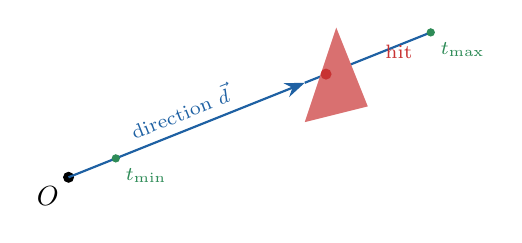
\begin{tikzpicture}
    \fill (0,0) circle (2pt) node[below left] {$O$};
    \draw[arr,rtblue] (0,0) -- (3,1.2) node[midway,above,sloped,font=\scriptsize] {direction $\vec d$};
    \draw[rtblue,thick] (3,1.2) -- (4.6,1.84);
    \fill[rtgreen] (0.6,0.24) circle (1.5pt) node[below right,font=\scriptsize] {$t_{\min}$};
    \fill[rtgreen] (4.6,1.84) circle (1.5pt) node[below right,font=\scriptsize] {$t_{\max}$};
    \fill[rtred!70] (3.0,0.7) -- (3.4,1.9) -- (3.8,0.9) -- cycle;
    \fill[rtred] (3.27,1.31) circle (2pt);
    \node[rtred,font=\scriptsize,right] at (3.9,1.6) {hit};
  \end{tikzpicture}
  \end{center}
  \begin{itemize}
    \item Ray--triangle test (M\"oller--Trumbore): a few dot/cross products; \alert{cheap, and done in hardware}.
    \item The difficulty is not one test, it is the \alert{number} of tests.
  \end{itemize}
\end{frame}

\begin{frame}{BVH: discard groups of triangles at once}
  \begin{columns}[T]
    \begin{column}{0.5\textwidth}
      \centering
      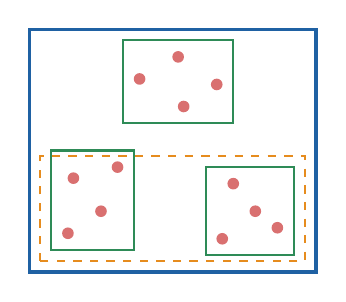
\begin{tikzpicture}[scale=0.7]
        \foreach \x/\y in {0.5/0.5,1.1/0.9,0.6/1.5,1.4/1.7,3.3/0.4,3.9/0.9,3.5/1.4,4.3/0.6,1.8/3.3,2.5/3.7,3.2/3.2,2.6/2.8}{\fill[rtred!70] (\x,\y) circle (3pt);}
        \draw[rtgreen,thick] (0.2,0.2) rectangle (1.7,2.0);
        \draw[rtgreen,thick] (3.0,0.1) rectangle (4.6,1.7);
        \draw[rtgreen,thick] (1.5,2.5) rectangle (3.5,4.0);
        \only<2->{\draw[rtorange,thick,dashed] (0.0,0.0) rectangle (4.8,1.9);
                  \draw[rtblue,very thick] (-0.2,-0.2) rectangle (5.0,4.2);}
      \end{tikzpicture}
    \end{column}
    \begin{column}{0.48\textwidth}
      \centering
      \only<2->{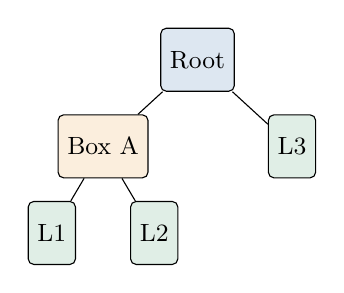
\begin{tikzpicture}[level distance=1.1cm,
          level 1/.style={sibling distance=2.4cm},
          level 2/.style={sibling distance=1.3cm},every node/.style={font=\scriptsize}]
        \node[box=rtblue] {Root}
          child { node[box=rtorange] {Box A}
            child { node[box=rtgreen] {L1} } child { node[box=rtgreen] {L2} } }
          child { node[box=rtgreen] {L3} };
      \end{tikzpicture}}
    \end{column}
  \end{columns}
  \begin{itemize}
    \item<1-> Group nearby triangles in axis-aligned boxes (leaves).
    \item<2-> Group boxes recursively: if a ray misses a box, it misses \alert{everything inside}.
    \item<3-> Traversal: test root, descend only into hit boxes, test triangles only in reached leaves. Built \alert{once}, used for millions of rays.
  \end{itemize}
\end{frame}

\begin{frame}{RT Cores: traversal in silicon}
  \begin{columns}[T]
    \begin{column}{0.5\textwidth}
      \begin{itemize}
        \item Each SM of an RTX GPU has an \alert{RT Core}: fixed-function unit walking the BVH.
        \item Ray--box and ray--triangle tests in hardware.
        \item CUDA cores only \alert{launch} the ray and read the result.
        \item Target here: \texttt{sm\_86} (Ampere).
      \end{itemize}
    \end{column}
    \begin{column}{0.48\textwidth}
      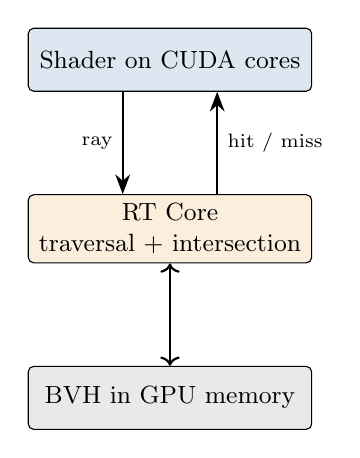
\begin{tikzpicture}
        \node[box=rtblue,minimum width=3.6cm] (sm) {Shader on CUDA cores};
        \node[box=rtorange,minimum width=3.6cm,below=1.3cm of sm] (rt) {RT Core\\traversal + intersection};
        \node[box=rtgray,minimum width=3.6cm,below=1.3cm of rt] (mem) {BVH in GPU memory};
        \draw[arr] ([xshift=-0.6cm]sm.south) -- node[left,font=\scriptsize] {ray} ([xshift=-0.6cm]rt.north);
        \draw[arr] ([xshift=0.6cm]rt.north) -- node[right,font=\scriptsize] {hit / miss} ([xshift=0.6cm]sm.south);
        \draw[arr,<->] (rt) -- (mem);
      \end{tikzpicture}
    \end{column}
  \end{columns}
\end{frame}

%=====================================================================
\section{OptiX and the algorithm}
%=====================================================================
\begin{frame}{OptiX: three notions are enough}
  OptiX: we write small programs, NVIDIA provides the BVH and the traversal.
  \begin{center}
  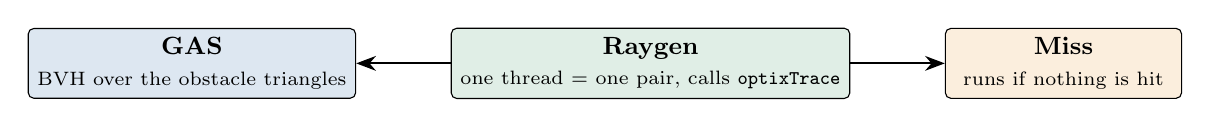
\begin{tikzpicture}[node distance=1.2cm]
    \node[box=rtblue,minimum width=3cm] (gas) {\textbf{GAS}\\\scriptsize BVH over the obstacle triangles};
    \node[box=rtgreen,minimum width=3cm,right=of gas] (rg) {\textbf{Raygen}\\\scriptsize one thread = one pair, calls \texttt{optixTrace}};
    \node[box=rtorange,minimum width=3cm,right=of rg] (ms) {\textbf{Miss}\\\scriptsize runs if nothing is hit};
    \draw[arr] (rg) -- (gas);
    \draw[arr] (rg) -- (ms);
  \end{tikzpicture}
  \end{center}
  \begin{itemize}
    \item The GAS contains \alert{only the obstacles}, as a triangle soup (3 vertices per triangle, no index buffer).
    \item Flags: \texttt{PREFER\_FAST\_TRACE} (many rays), \texttt{DISABLE\_ANYHIT}.
    \item Other pieces (pipeline, SBT, PTX) are only plumbing: see the interfacing part.
  \end{itemize}
\end{frame}

\begin{frame}{Running example: $N=5$, one obstacle}
  \begin{columns}[T]
    \begin{column}{0.45\textwidth}
      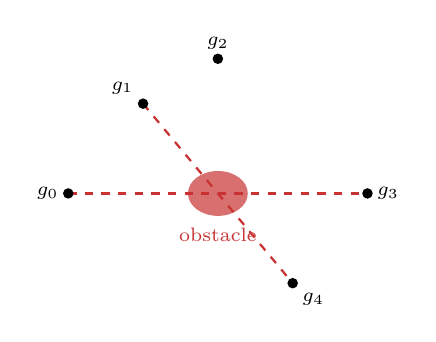
\begin{tikzpicture}[scale=0.95]
        \fill[rtred!70] (0,0) ellipse (0.4 and 0.3);
        \node[rtred,font=\scriptsize] at (0,-0.55) {obstacle};
        \coordinate (p0) at (-2,0); \coordinate (p1) at (-1,1.2); \coordinate (p2) at (0,1.8);
        \coordinate (p3) at (2,0);  \coordinate (p4) at (1,-1.2);
        \draw[rtred,dashed,thick] (p0)--(p3);
        \draw[rtred,dashed,thick] (p1)--(p4);
        \foreach \n/\a in {0/left,1/above left,2/above,3/right,4/below right}{
          \fill (p\n) circle (2pt) node[\a,font=\scriptsize] {$g_\n$};}
      \end{tikzpicture}
    \end{column}
    \begin{column}{0.53\textwidth}
      \begin{itemize}
        \item 5 points, 10 pairs, 10 rays.
        \item Blocked: $(0,3)$ and $(1,4)$.
        \item We will follow this case through indexing, kernel and bitset.
      \end{itemize}
      \vspace{2mm}
      \small
      \begin{tabular}{c|cccccccccc}
        $k$ & 0&1&2&3&4&5&6&7&8&9\\ \hline
        $(i,j)$ & 01&02&03&04&12&13&14&23&24&34\\
        bit & 1&1&\alert{0}&1&1&1&\alert{0}&1&1&1
      \end{tabular}
    \end{column}
  \end{columns}
\end{frame}

\begin{frame}{One pair = one index $k$}
  One thread per pair $(i,j)$, $i<j$, numbered row by row in the upper triangle (here $N=5$, 10 pairs).
  \begin{columns}[T]
    \begin{column}{0.4\textwidth}
      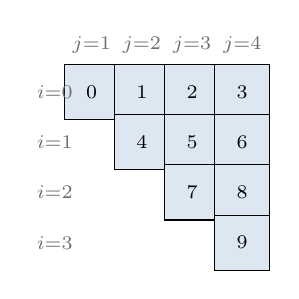
\begin{tikzpicture}[scale=0.85]
        \foreach \i/\j/\k in {0/1/0,0/2/1,0/3/2,0/4/3,1/2/4,1/3/5,1/4/6,2/3/7,2/4/8,3/4/9}{
          \node[draw,fill=rtblue!15,minimum size=0.7cm,font=\scriptsize] at (\j*0.75,-\i*0.75) {\k};}
        \foreach \i in {0,...,3}{\node[font=\scriptsize,rtgray] at (0.2,-\i*0.75) {$i{=}\i$};}
        \foreach \j in {1,...,4}{\node[font=\scriptsize,rtgray] at (\j*0.75,0.7) {$j{=}\j$};}
      \end{tikzpicture}
    \end{column}
    \begin{column}{0.58\textwidth}
      \[ \text{rowOffset}(i)=\frac{i\,(2N-i-1)}{2} \]
      \[ i=\Bigl\lfloor \tfrac{(2N-1)-\sqrt{(2N-1)^2-8k}}{2}\Bigr\rfloor,\quad j=k-\text{rowOffset}(i)+i+1 \]
      \begin{itemize}
        \item \texttt{double} square root + \texttt{while} corrections against rounding.
        \item $O(1)$ memory per thread: no $N\times N$ table.
      \end{itemize}
    \end{column}
  \end{columns}
\end{frame}

\begin{frame}[fragile]{The raygen program (1/2): which pair, which ray}
\begin{lstlisting}
extern "C" __global__ void __raygen__rg() {
  @const unsigned long long k = params.k0 + optixGetLaunchIndex().x;@
  if (k >= params.numPairs) return;
  @unsigned a, b;  unrank(k, params.N, a, b);       // k -> (i,j)@

  @float3 P = params.pts[a], Q = params.pts[b];@
  @float3 d = Q - P;  float L = sqrtf(dot3(d,d));   // segment length@
  d /= L;                                          // unit direction
  ...
}
\end{lstlisting}
  \begin{itemize}
    \item Red: map the thread to a pair, then build the segment $P\to Q$ as a ray.
    \item \texttt{params.pts}: the offset origins $O_i=g_i+\delta\vec n$ (see interfacing).
  \end{itemize}
\end{frame}

\begin{frame}[fragile]{The raygen program (2/2): trace and write}
\begin{lstlisting}
  @unsigned occluded = 1;                           // pessimistic@
  optixTrace(params.gas, P, d,
             @params.tminRel*L, params.tmaxRel*L, 0.0f,@
             OptixVisibilityMask(255),
             @TERMINATE_ON_FIRST_HIT | DISABLE_CLOSESTHIT,@
             0, 1, 0, occluded);
  @if (!occluded) atomicOr(&params.bits[k >> 5], 1u << (k & 31));@
\end{lstlisting}
  \begin{columns}[T]
    \begin{column}{0.56\textwidth}
      \begin{itemize}
        \item Interval $[10^{-6}L,\,(1-10^{-5})L]$: starts just after $P$, stops just before $Q$.
        \item \alert{Pessimistic payload}: \texttt{occluded}=1; only the \texttt{miss} program sets it to 0. A hit runs nothing: fastest path.
        \item \texttt{atomicOr}: 32 threads write the same 32-bit word.
      \end{itemize}
    \end{column}
    \begin{column}{0.4\textwidth}
      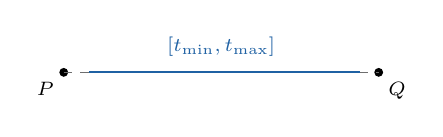
\begin{tikzpicture}[scale=0.8]
        \fill (0,0) circle (2pt) node[below left,font=\scriptsize] {$P$};
        \fill (5,0) circle (2pt) node[below right,font=\scriptsize] {$Q$};
        \draw[rtblue,thick] (0.4,0) -- (4.7,0);
        \node[font=\scriptsize,rtblue,above] at (2.5,0.1) {$[t_{\min},t_{\max}]$};
        \draw[rtgray,dashed] (0,0)--(0.4,0); \draw[rtgray,dashed] (4.7,0)--(5,0);
      \end{tikzpicture}
    \end{column}
  \end{columns}
\end{frame}


\begin{frame}{Bitset, chunks, and back to the running example}
  \begin{columns}[T]
    \begin{column}{0.5\textwidth}
      \begin{itemize}
        \item 1 bit per pair: word \texttt{k>>5}, bit \texttt{k\&31}.
        \item Memory $N(N-1)/16$ bytes instead of $8N^2$: factor $\approx 128$.
        \item One \texttt{optixLaunch} is limited ($\leq 2^{30}$): chunks of $2^{28}$ pairs, offset \texttt{k0}.
      \end{itemize}
    \end{column}

    \begin{column}{0.48\textwidth}
      \centering
      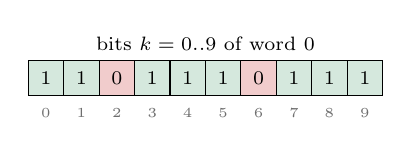
\begin{tikzpicture}[scale=0.9]
        \foreach \x/\b in {0/1,1/1,2/0,3/1,4/1,5/1,6/0,7/1,8/1,9/1}{
          \ifnum\b=0
            \def\bitcolor{rtred!25}
          \else
            \def\bitcolor{rtgreen!20}
          \fi

          \draw[fill=\bitcolor] (\x*0.5,0) rectangle +(0.5,0.5);
          \node[font=\scriptsize] at (\x*0.5+0.25,0.25) {\b};
          \node[font=\tiny,rtgray] at (\x*0.5+0.25,-0.25) {\x};
        }

        \node[font=\scriptsize,above] at (2.5,0.5)
          {bits $k=0..9$ of word 0};
      \end{tikzpicture}

      \vspace{3mm}
      $\Downarrow$ unpack ($V_{ij}=V_{ji}=\text{bit}(k)$, $V_{ii}=0$)

      \vspace{1mm}
      $V=\begin{pmatrix}
      0&1&1&0&1\\
      1&0&1&1&0\\
      1&1&0&1&1\\
      0&1&1&0&1\\
      1&0&1&1&0
      \end{pmatrix}$
    \end{column}
  \end{columns}
\end{frame}

%=====================================================================
\section{Interfacing FreeFEM++ $\leftrightarrow$ CUDA/OptiX}
%=====================================================================
\begin{frame}{Data flow}
  \begin{center}
  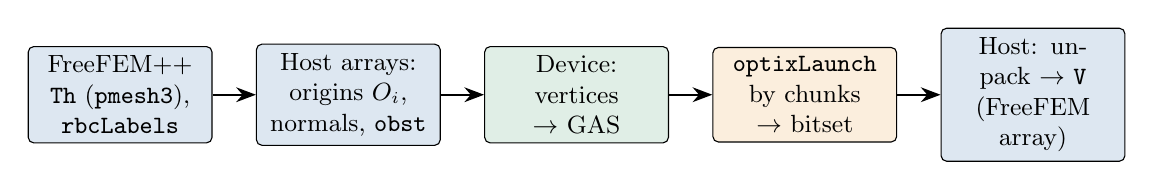
\begin{tikzpicture}[node distance=0.55cm,font=\scriptsize]
    \node[box=rtblue,text width=2.1cm] (a) {FreeFEM++ \texttt{Th} (\texttt{pmesh3}), \texttt{rbcLabels}};
    \node[box=rtblue,text width=2.1cm,right=of a] (b) {Host arrays: origins $O_i$, normals, \texttt{obst}};
    \node[box=rtgreen,text width=2.1cm,right=of b] (c) {Device: vertices $\to$ GAS};
    \node[box=rtorange,text width=2.1cm,right=of c] (d) {\texttt{optixLaunch} by chunks $\to$ bitset};
    \node[box=rtblue,text width=2.1cm,right=of d] (e) {Host: unpack $\to$ \texttt{V} (FreeFEM array)};
    \draw[arr] (a)--(b); \draw[arr] (b)--(c); \draw[arr] (c)--(d); \draw[arr] (d)--(e);
  \end{tikzpicture}
  \end{center}
  \textbf{CPU preparation, per boundary triangle $i$:}
  \begin{itemize}
    \item Barycenter $g_i$, unit normal $\vec n$, oriented \alert{inward} (adjacent tetrahedron, \texttt{BoundaryElement}).
    \item Origin $O_i=g_i+\delta\vec n$, $\delta=10^{-3}\sqrt{\text{area}}$: avoids \alert{self-intersection} if triangle $i$ is itself an obstacle.
    \item If its label is in \texttt{rbcLabels}: its 3 vertices go to \texttt{obst}. Empty \texttt{obst} is forbidden: insert a degenerate triangle at $10^{30}$.
  \end{itemize}
\end{frame}

\begin{frame}{Plugging into FreeFEM++}
  \begin{columns}[T]
    \begin{column}{0.5\textwidth}
      \begin{itemize}
        \item Exposed with \texttt{LOADFUNC}; called from the \texttt{.edp} script:\\
        \texttt{OptixBuildVisibilityPairs3D(Th, rbcLabels, V)}
        \item \texttt{params.h}: the \texttt{Params} struct, shared by host (\texttt{.cpp}) and device (\texttt{.cu}).
        \item Device code compiled separately: \texttt{nvcc -ptx} $\to$ \texttt{.ptx}, loaded at runtime into the OptiX module/pipeline, with the SBT (program table).
      \end{itemize}
    \end{column}
    \begin{column}{0.48\textwidth}
      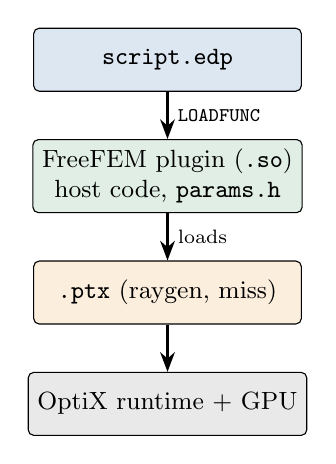
\begin{tikzpicture}[node distance=0.6cm,font=\scriptsize]
        \node[box=rtblue,minimum width=3.4cm] (edp) {\texttt{script.edp}};
        \node[box=rtgreen,minimum width=3.4cm,below=of edp] (so) {FreeFEM plugin (\texttt{.so}) \\ host code, \texttt{params.h}};
        \node[box=rtorange,minimum width=3.4cm,below=of so] (ptx) {\texttt{.ptx} (raygen, miss)};
        \node[box=rtgray,minimum width=3.4cm,below=of ptx] (gpu) {OptiX runtime + GPU};
        \draw[arr] (edp)--node[right]{\texttt{LOADFUNC}}(so);
        \draw[arr] (so)--node[right]{loads}(ptx);
        \draw[arr] (ptx)--(gpu);
      \end{tikzpicture}
    \end{column}
  \end{columns}
\end{frame}

\begin{frame}{Build chain}
  \begin{center}
  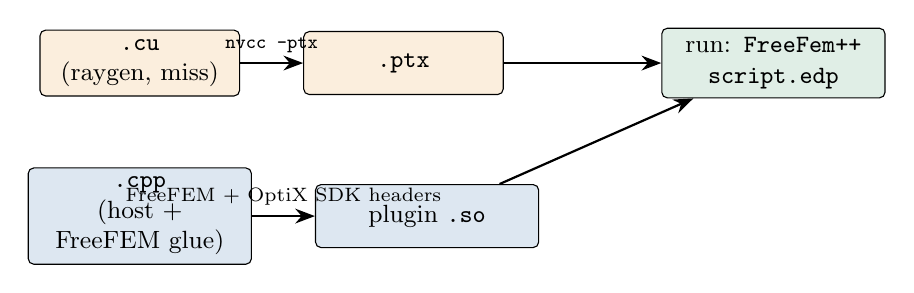
\begin{tikzpicture}[node distance=0.8cm,font=\scriptsize]
    \node[box=rtorange,text width=2.3cm] (cu) {\texttt{.cu}\\(raygen, miss)};
    \node[box=rtorange,text width=2.3cm,right=of cu] (ptx) {\texttt{.ptx}};
    \node[box=rtblue,text width=2.6cm,below=0.9cm of cu] (cpp) {\texttt{.cpp}\\(host + FreeFEM glue)};
    \node[box=rtblue,text width=2.6cm,right=of cpp] (so) {plugin \texttt{.so}};
    \node[box=rtgreen,text width=2.6cm,right=2cm of ptx] (run) {run: \texttt{FreeFem++ script.edp}};
    \draw[arr] (cu)--node[above]{\texttt{nvcc -ptx}}(ptx);
    \draw[arr] (cpp)--node[above]{FreeFEM + OptiX SDK headers}(so);
    \draw[arr] (ptx)--(run); \draw[arr] (so)--(run);
  \end{tikzpicture}
  \end{center}
  \begin{itemize}
    \item Requirements: OptiX SDK headers, CUDA toolkit, RTX GPU, FreeFEM++ plugin toolchain (\textbf{TODO}: exact commands/versions).
    \item The \texttt{.ptx} must sit in the working directory, with the name of the compiled \texttt{.cu}.
  \end{itemize}
\end{frame}

%=====================================================================
\section{Application and results}
%=====================================================================
\begin{frame}{Validation}
  \begin{columns}[T]
    \begin{column}{0.5\textwidth}
      \begin{itemize}
        \item Small mesh: compare $V$ with a CPU reference (brute-force M\"oller--Trumbore).
        \item Check: symmetry, zero diagonal, number of mismatches.
        \item Sensitivity to $\delta$, $t_{\min}$, $t_{\max}$ (\texttt{float} precision).
      \end{itemize}
      \textbf{TODO}: report mismatch count (expected: 0 or only grazing rays).
    \end{column}
    \begin{column}{0.48\textwidth}
      \figplaceholder{visibility_from_triangle.png}{\textwidth}{Visibility from one triangle: visible triangles in green, blocked in red}
    \end{column}
  \end{columns}
\end{frame}

\begin{frame}{Performance}
  \begin{columns}[T]
    \begin{column}{0.5\textwidth}
      \figplaceholder{benchmark.pdf}{\textwidth}{Time vs.\ $N$: GPU OptiX vs.\ CPU brute force vs.\ CPU BVH (log--log)}
    \end{column}
    \begin{column}{0.48\textwidth}
      \begin{itemize}
        \item Fill in: GPU model, $N$, $M$, times, speed-up.
        \item Break down: CPU preparation / GAS build / launches / copy-back and unpack.
        \item Is the bottleneck the GPU, or the host-side loop?
      \end{itemize}
    \end{column}
  \end{columns}
\end{frame}

\begin{frame}{Using $V$ in the simulation}
  \begin{itemize}
    \item \textbf{TODO}: describe how $V$ enters the FreeFEM++ problem (assembly of the coupling, time loop, mesh deformation?).
    \item Is $V$ recomputed at each step (moving cells) or once? This decides the relevance of GPU speed.
    \item Show a physical result (field, flux, comparison with/without occlusion).
  \end{itemize}
  \vspace{3mm}
  \figplaceholder{application_result.png}{0.6\textwidth}{Simulation result using $V$}
\end{frame}

%=====================================================================
\section{Conclusion}
%=====================================================================
\begin{frame}{Limits and perspectives}
  \begin{itemize}
    \item \alert{Precision}: geometry in \texttt{float}; $\delta$, $t_{\min}$, $t_{\max}$ are compromises to validate on real meshes.
    \item \alert{Memory}: bitset grows as $N^2$; beyond a few $10^5$ triangles, process by blocks of rows.
    \item \alert{Orientation tests} (faces looking at each other) currently disabled: only occlusion counts. Re-enabling them would also discard useless rays.
    \item Perspectives: dynamic meshes (BVH refit/update), multi-GPU, view factors with weights instead of 0/1.
  \end{itemize}
\end{frame}

\begin{frame}{Key takeaways}
  \begin{enumerate}
    \item Visibility = one \alert{ray vs.\ obstacles} query per pair; rays are \alert{independent}.
    \item A \alert{BVH} (GAS) discards most triangles; \alert{RT Cores} traverse it in hardware.
    \item \alert{OptiX}: GAS + raygen + miss; pessimistic payload = fastest occlusion test.
    \item \alert{Triangular indexing} halves the work; the \alert{bitset} cuts memory by $\approx128$.
    \item Interfacing: \texttt{LOADFUNC} plugin + \texttt{.ptx} loaded at runtime.
  \end{enumerate}
  \vspace{2mm}
  \centering Thank you --- questions?
\end{frame}

%=====================================================================
\appendix
\section{Backup}
\begin{frame}{Backup: known issue (host-side overflow)}
  \begin{itemize}
    \item In the final unpack loop, \texttt{int base} and \texttt{int k} overflow $2^{31}$ as soon as $N\gtrsim65\,000$. Use \texttt{unsigned long long}.
    \item Likewise \texttt{i*nbe+j} is computed in \texttt{int} before indexing \texttt{V}: cast to \texttt{size\_t}.
  \end{itemize}
\end{frame}

\begin{frame}{Backup: OptiX details}
  \begin{itemize}
    \item \textbf{IAS} (instance acceleration structure): for multi-object scenes; unnecessary here, hence \texttt{ALLOW\_SINGLE\_GAS}.
    \item \textbf{Hit group}: present but empty; \texttt{DISABLE\_CLOSESTHIT} and \texttt{DISABLE\_ANYHIT} skip it.
    \item \textbf{SBT}: table telling OptiX which raygen / miss / hit-group program to call.
    \item Mask 255: ray sees all geometry.
  \end{itemize}
\end{frame}

\begin{frame}{\textcolor{white}{Motivation: why ray tracing?}}
  \begin{columns}[T]
    \begin{column}{0.55\textwidth}
      \medskip
      \textbf{Current cost.} For every value of $\kappa$, assemble
      \[
        G^{ij}_\kappa=\frac{1}{4\pi}\int_\Omega
        \kappa\,\frac{e^{-\int_{[\bol{x}^i,\bol{x}']}\kappa}}{|\bol{x}^i-\bol{x}'|^2}\,\hat w^j(\bol{x}')\dd\bol{x}'
      \]
      \vspace{-0.4em}
      \begin{itemize}
        \item $\sim 10^6$ vertices, $2\times$ (\#values of $\kappa$) $\mathcal H$-matrices
        \item every entry needs a \textbf{line integral} of $\kappa$
        \item volume assembly: $\sim$ 130 s on 384 cores
      \end{itemize}
      \medskip
      \textbf{Idea.} In a valley, most pairs $(\bol{x},\bol{x}')$ do not see each other: use \textbf{ray tracing} to avoid computing them.
    \end{column}
    \begin{column}{0.41\textwidth}
      \centering
      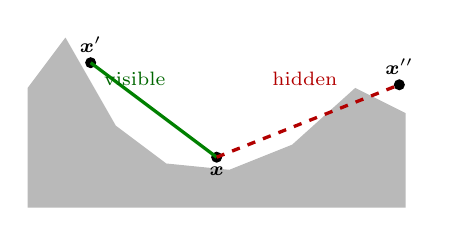
\begin{tikzpicture}[scale=0.8]
        \fill[gray!55] (0,-0.3) -- (0,1.6) -- (0.6,2.4) -- (1.4,1.0) -- (2.2,0.4) -- (3.2,0.3) -- (4.2,0.7) -- (5.2,1.6) -- (6,1.2) -- (6,-0.3) -- cycle;
        \fill (3,0.5) circle (2.5pt) node[below] {\scriptsize $\bol{x}$};
        \fill (1,2.0) circle (2.5pt) node[above] {\scriptsize $\bol{x}'$};
        \fill (5.9,1.65) circle (2.5pt) node[above] {\scriptsize $\bol{x}''$};
        \draw[green!50!black, very thick] (3,0.5) -- (1,2.0);
        \draw[red!70!black, very thick, dashed] (3,0.5) -- (5.9,1.65);
        \node[red!70!black, font=\scriptsize] at (4.4,1.75) {hidden};
        \node[green!40!black, font=\scriptsize] at (1.7,1.75) {visible};
      \end{tikzpicture}

      \smallskip
      {\footnotesize \textcolor{green!40!black}{green}: computed \quad
      \textcolor{red!70!black}{red}: skipped}
    \end{column}
  \end{columns}
\end{frame}

\begin{frame}{\textcolor{white}{Radiative transfer: what is the goal?}}
  \begin{columns}[T]
    \begin{column}{0.55\textwidth}
      \medskip
      \textbf{Goal:} compute the temperature $T(\bol{x})$ in the atmosphere, driven by radiation.
      \vspace{0.3em}
      \begin{itemize}
        \item \textbf{Sun}: short waves, atmosphere mostly transparent
        \item \textbf{Earth}: long waves (infrared), absorbed and re-emitted by air, clouds, CO$_2$, contrails
        \item \textbf{Terrain} matters: mountains and valleys $\Rightarrow$ full 3D geometry
      \end{itemize}
      \vspace{0.3em}
      \[
        \bol{\omega}\cdot\nabla I_\nu+\kappa_\nu I_\nu=\kappa_\nu B_\nu(T)
        \;\;\longleftrightarrow\;\; T
      \]
      \vspace{-0.6em}
      \begin{center}
        \textcolor{red!70!black}{\textbf{Costly:}} $I_\nu(\bol{x},\bol{\omega})$ depends on 7 variables
      \end{center}
    \end{column}
    \begin{column}{0.41\textwidth}
      \centering
      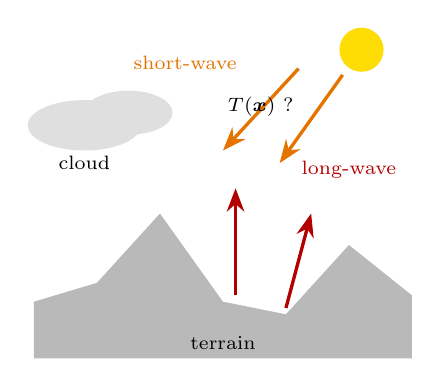
\begin{tikzpicture}[scale=0.8]
        % terrain
        \fill[gray!55] (0,-0.3) -- (0,0.6) -- (1,0.9) -- (2,2.0) -- (3,0.6) -- (4,0.4) -- (5,1.5) -- (6,0.7) -- (6,-0.3) -- cycle;
        % sun
        \fill[yellow!80!orange] (5.2,4.6) circle (0.35);
        \draw[orange!90!black, very thick, -{Stealth}] (4.9,4.2) -- (3.9,2.8);
        \draw[orange!90!black, very thick, -{Stealth}] (4.2,4.3) -- (3.0,3.0);
        % cloud
        \fill[gray!25] (0.8,3.4) ellipse (0.9 and 0.4);
        \fill[gray!25] (1.5,3.6) ellipse (0.7 and 0.35);
        % infrared from the ground
        \draw[red!70!black, very thick, -{Stealth}] (3.2,0.7) -- (3.2,2.4);
        \draw[red!70!black, very thick, -{Stealth}] (4.0,0.5) -- (4.4,2.0);
        % labels
        \node[orange!90!black, font=\scriptsize] at (2.4,4.4) {short-wave};
        \node[red!70!black, font=\scriptsize] at (5.0,2.7) {long-wave};
        \node[font=\scriptsize] at (0.8,2.8) {cloud};
        \node[font=\scriptsize] at (3.0,-0.05) {terrain};
        \node[font=\scriptsize] at (3.6,3.7) {$T(\bol{x})$ ?};
      \end{tikzpicture}
    \end{column}
  \end{columns}
\end{frame}

\end{document}